\documentclass[../main.tex]{subfiles}
    
\begin{document}
The GUI (RF-2) and TTS (RF-3) was successfully along with the OCR\@. For blank papers with black text, the preprocessing tend to successfully remove color from pixels that are not part of the text. Figure~\ref{fig:alphabet} and Figure~\ref{fig:straight} shows examples of images before (a) and after preprocessing (b). The accuracy of similar images tend to be \~80--95\%. The accuracy for those specific examples are 85\% for Figure~\ref{fig:alphabet} and 99\% for Figure~\ref{fig:straight}.

\begin{figure}[h!]
  \centering
  \begin{subfigure}[t]{0.48\linewidth}
    \centering
    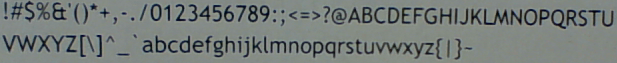
\includegraphics[width=\textwidth]{alphabet_raw}
    \caption{Raw input image\label{fig:alphabet_a}}
  \end{subfigure}~
  \begin{subfigure}[t]{0.48\linewidth}
    \centering
    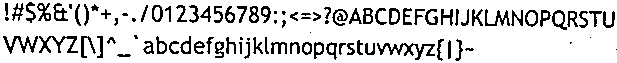
\includegraphics[width=\textwidth]{alphabet_processed}
    \caption{Image after processing\label{fig:alphabet_b}}
  \end{subfigure}
  \caption{Text recognised with 85\% accuracy.\label{fig:alphabet}}
\end{figure}

\begin{figure}[h!]
  \centering
  \begin{subfigure}[t]{0.48\linewidth}
    \centering
    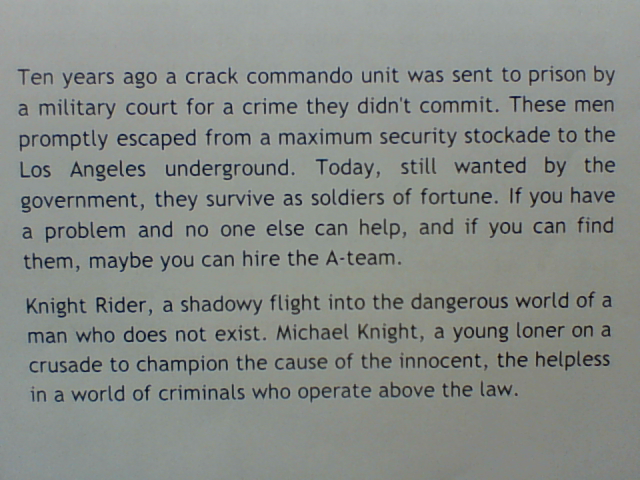
\includegraphics[width=\textwidth]{straight_raw}
    \caption{Raw input image\label{fig:straight_a}}
  \end{subfigure}~
  \begin{subfigure}[t]{0.48\linewidth}
    \centering
    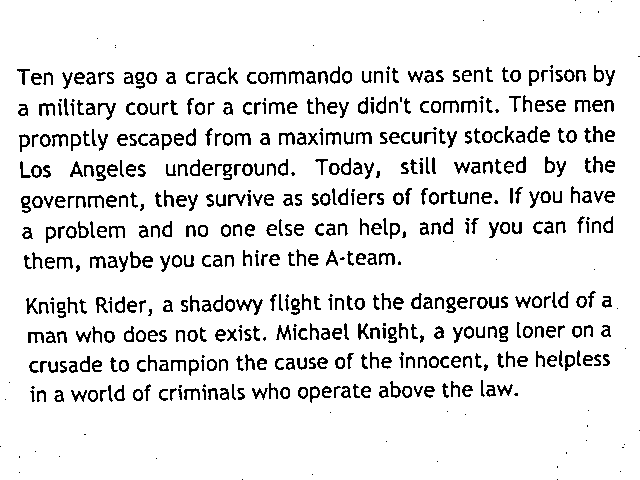
\includegraphics[width=\textwidth]{straight_processed}
    \caption{Image after processing\label{fig:straight_b}}
  \end{subfigure}
  \caption{Text recognised with 99\% accuracy.\label{fig:straight}}
\end{figure}

On a skewed text, the performance is significantly worse. The skewed text in Figure~\ref{fig:skewed}, is clear and readable for a human, but tesseract only recognised 12 words correctly out of the entire text. The second paragraph was not even recognised as text. 

\begin{figure}[h!]
  \centering
  \begin{subfigure}[t]{0.48\linewidth}
    \centering
    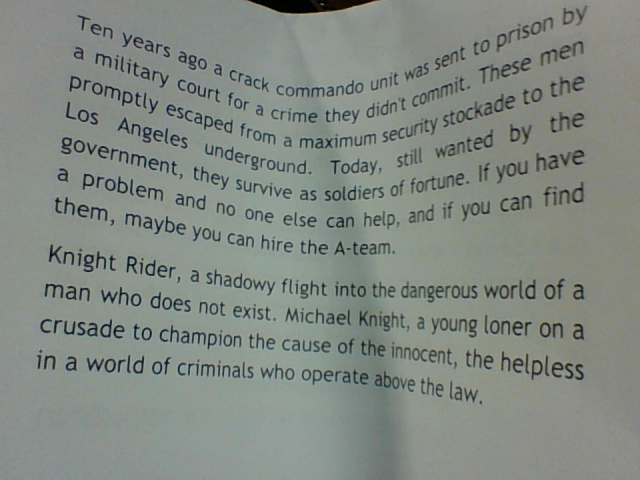
\includegraphics[width=\textwidth]{skewed_raw}
    \caption{Raw input image\label{fig:skewed_a}}
  \end{subfigure}~
  \begin{subfigure}[t]{0.48\linewidth}
    \centering
    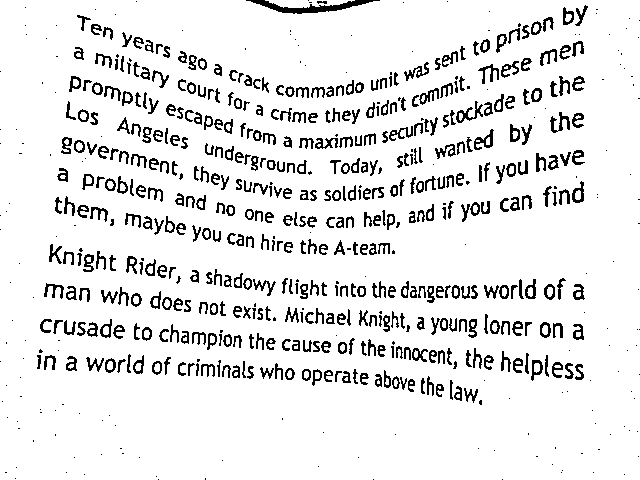
\includegraphics[width=\textwidth]{skewed_processed}
    \caption{Image after processing\label{fig:skewed_b}}
  \end{subfigure}
  \caption{Text with low recognition accuracy.\label{fig:skewed}}
\end{figure}

The definition accuracy was found to be too ambiguous to tell whether RF-1 and OF-3 from Table~\ref{table:specs} was achieved or not. The result is too dependent on the input.

\end{document}